% 拉格朗日乘数法
% 多元微积分|导数|极值|梯度|拉格朗日函数|拉格朗日乘数法

\pentry{导数与函数极值\upref{DerMax}, 梯度\upref{Grad}}

若要求函数 $f(x_1,\dots, x_N)$ 在 $m$ 个约束条件 $g_i(x_1, \dots, x_N)\ \ (i = 1,\dots, M)$ 下的极值, 可用拉格朗日乘数法, 令拉格朗日函数为
\begin{equation}
\Lambda(x_1,\dots, x_N) = f + \sum_{i=1}^M \lambda_i g_i
\end{equation} 
其中 $\lambda_i$ 为未知任意常数. 同时满足约束条件和
\begin{equation}
\pdv{\Lambda}{x_i} = 0 \quad (i = 1,\dots, N)
\end{equation}
的点, 就是函数 $f(x_1, \dots, x_N)$ 的极值点或稳定点.

\subsection{几何理解}

下面举一个二元函数的例子以说明拉格朗日乘数法的几何意义.

\begin{figure}[ht]
\centering
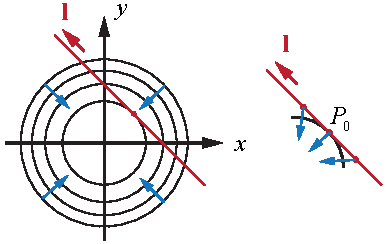
\includegraphics[width=6cm]{./figures/LagMul_1.pdf}
\caption{\autoref{LagMul_ex1} } \label{LagMul_fig1}
\end{figure}

\begin{example}{}\label{LagMul_ex1}
求函数 $f(x,y) = -a(x^2 + y^2)$ 在轨迹 $x+y = c$ 约束下的最值($a,c$ 均为常数).

从几何上来理解, 函数 $f(x,y)$ 是一个倒置的抛物面, 其等高线的俯视图如\autoref{LagMul_fig1} 蓝色的箭头代表函数值增加最大的方向, 即梯度的方向. 考察点沿着同一条等高线的位置变化时, 函数值不变. 曲面上任意一点的梯度为
\begin{equation}
\grad f = \pdv{f}{x} \uvec x + \pdv{f}{y} \uvec y = -2ax\uvec x -2ay\uvec y = -2a\bvec r
\end{equation}
其中 $\bvec r$ 为位矢. 这说明, 梯度的方向总是延径向向内, 与距离成正比.

约束条件如\autoref{LagMul_fig1} 中红线所示, 我们要求的就是红线上面函数 $f$ 的极值. 在该题的情况下, 所求的极值显然在红线离原点最近的地方出现.

但是如何总结出约束条件下多元函数极值点的一般的判断条件并用梯度表示呢? 根据梯度的性质(\autoref{Grad_eq5}~\upref{Grad}), 如果考察点沿红线的切向移动 $\dd{\bvec l}$, 函数值的微分为
\begin{equation}
\dd{f} = \grad f\vdot \dd{\bvec l}
\end{equation}
使用导数和极值的关系\upref{DerMax}, 我们要找的极值点满足: 函数在极值点处延红线切向的方向导数为零. 即
\begin{equation}
\grad f \vdot \dd{\bvec l} = 0
\end{equation}
这说明 $\grad f$ 只可能具有极值点处红线的法向量分量而切向分量为 0, 即 $\grad f$ 与法向量共线. 令约束条件即红线的方程为
\begin{equation}
g(x, y) = x+y-c = 0
\end{equation}
$g(x,y)$ 的梯度就是其法向量.%链接未完成
由矢量共线的定义,%链接未完成
存在常数 $\lambda$, 使
\begin{equation}
\grad f + \lambda \grad g = 0 \qquad \text{即} \qquad \grad(f + \lambda g) = 0
\end{equation}
这就是拉格朗日乘数法. 其中 $f + \lambda g$ 就是拉格朗日函数. 下面根据该条件, 对本题进行求解. 本题中拉格朗日函数梯度的两个分量分别为
\begin{equation}\ali{
0 &= \pdv{x} (f + \lambda g) = -2ax + \lambda\\
0 &= \pdv{y} (f + \lambda g) = -2ay + \lambda
}\end{equation}
两式消去 $\lambda$, 得 $x = y$. 再结合约束条件 $x + y - c = 0$, 得极值点为 $(c/2, c/2)$. 可见拉格朗日乘数法求出的偏导条件并没有包含约束条件, 而是需要再次联立约束条件才可以得出最后答案.
\end{example}

以上的推导可以很容易地拓展到多元函数和多个限制条件中去. 例如求三元函数 $f(x,y,z)$ 中(可看作空间的标量场), 在两个约束条件 $g_1(x,y,z) = 0, g_2(x,y,z) = 0$ 下的极值. 注意两个约束条件分别代表一个曲面, 同时成立代表两个曲面相交的空间曲线. 我们要在该曲线上求函数 $f$ 的极值. 同样, 若曲线上的某点是极值, 那必须满足曲线在该点的切线方向 $f$ 的方向导数为零, 即 $\grad f$ 与该点法向量共线. 然而这是个三维问题, 空间曲线的任意一点可以有两条不共线的法向量(不一定互相垂直), 该点的任何其他法向量可以由这两个法线的线性组合来表示. 即存在常数 $\lambda_1$ 和 $\lambda_2$, 使得
\begin{equation}
\grad f + \lambda_1 \grad g_1 + \lambda_2 \grad g_2 = 0
\end{equation}
即
\begin{equation}
\grad (f + \lambda_1 g_1 + \lambda_2 g_2) = 0
\end{equation}
其中 $f + \lambda_1 g_1 + \lambda_2 g_2$ 就是拉格朗日函数. 当然, 限制条件的数目不一定是2, 若只有一个限制条件 $g_1 = 0$, 就是求曲面 $g_1 = 0$ 上函数 $f$ 取得极值的点, 条件是函数的梯度 $\grad f$ 与曲面的法向量 $\grad g_1$ 共线.

\begin{example}{}
椭圆方程为 $x^2/a^2 + y^2/b^2 = 1$, 求其内接长方型的最大面积(长方形的边平行于 $x$ 轴和 $y$ 轴).

令长方型的右上角与椭圆的切点为 $(x,y)$, 则长方型的面积为 $S = 4xy$. 约束函数为 $g = x^2/a^2 + y^2/b^2 - 1$. 拉格朗日函数为
\begin{equation}
\Lambda(x,y) = S + \lambda g = 4xy + \lambda \qty(\frac{x^2}{a^2} + \frac{y^2}{b^2} - 1)
\end{equation}
令 $x, y$ 偏导都为 0, 得
\begin{equation}
\begin{cases}
4y + 2\lambda x/a^2 = 0\\
4x + 2\lambda y/b^2 = 0
\end{cases}
\end{equation}
两式消去 $\lambda$, 得 $x/y = a/b$. 再联立椭圆方程, 解得 $(x,y) = (a/\sqrt{2}, b/\sqrt{2})$, 面积最大值为 $2ab$.
\end{example}
